\documentclass[conference]{IEEEtran}

\usepackage[utf8]{inputenc}
\usepackage[T1]{fontenc}
\usepackage{amsmath,amssymb,amsfonts,bm}
\usepackage{graphicx}
\graphicspath{{figures/}{./}}
\usepackage{booktabs}
\usepackage{array}
\usepackage{cite}
\usepackage{url}
\usepackage[hidelinks]{hyperref}
\usepackage{tikz}
\usetikzlibrary{arrows.meta,positioning,fit}

\newcommand{\method}{PRISM-XAI}
\newcommand{\mapxai}{MAP-XAI}
\newcommand{\E}{\mathbb{E}}

\begin{document}

\title{PRISM-XAI: Privacy-Accounted Semantic Explanation Scheduling for Smart-Grid Edge Intelligence}
\author{\IEEEauthorblockN{Author information available in the submission system}}

\maketitle

\begin{abstract}
Repeatedly delivering household-level explanations can help a grid
operator understand rapid demand changes, but explanation packets consume
wireless resources and may reveal private behaviour. We introduce
\emph{PRISM-XAI}, a two-layer design for privacy-accounted semantic
explanation delivery. The first layer, Multi-level Adaptive Privacy for
XAI (\mapxai{}), converts explanation changes into compact private
semantic packets: an endpoint clips an attribution delta, applies a
Gaussian differential-privacy (DP) mechanism, and only then performs
Top-$k$ selection and quantization while a R\'enyi-DP accountant tracks
cumulative household privacy. The second layer, \method{}, decides
whether, when, from which endpoint, and at what resolution those packets
should be transmitted using channel state, packet deadline, Age of
Explanation (AoX), public grid criticality, endpoint fairness, residual
signal, and expected fidelity gain per bit. In 720 paired runs on two
public electricity-demand datasets, two attribution methods, three
privacy budgets, six schedulers, and 10 seeds, the proposed stack incurs
no privacy-budget violations. At the selective-release operating point,
\method{} reduces explanation traffic by 79.4\% relative to joint
full-packet delivery and by about 94.6\% relative to fixed-DP schedulers,
with significantly lower traffic in all 48 paired external-baseline
comparisons. A feasibility ladder shows that Top-$K$ overlap remains
0.990/0.993 after clipping but falls to 0.241/0.282 after cumulative DP;
subsequent compression changes it only to 0.252/0.295. Thus, the dominant
fidelity bottleneck is repeated household-level privacy expenditure, not
semantic compression, motivating selective private release rather than
further compression-only tuning.
\end{abstract}

\begin{IEEEkeywords}
smart-grid communications, edge intelligence, explainable AI,
differential privacy, semantic communications, resource allocation,
Age of Explanation
\end{IEEEkeywords}

\section{Introduction}

Short-term load forecasts are more useful when an operator can also see
which factors drove the prediction. A demand surge caused by heating may
require a different response from one driven by electric-vehicle
charging or an unusual subset of customers. Feature-attribution methods
such as SHAP~\cite{lundberg2017shap} and Integrated Gradients
~\cite{sundararajan2017ig} can provide this evidence, and explainable AI
(XAI) is increasingly studied for load forecasting and grid monitoring
~\cite{bolstad2022load,wu2022load,kruse2021frequency,baur2024loadxai}.

Repeated explanation delivery creates a communication--privacy problem
that is different from evaluating XAI offline. First, household
attributions can leak information about private behaviour; explanations
are themselves potential privacy channels~\cite{shokri2021privacy}.
Second, transmitting every explanation in full consumes scarce uplink
capacity and may miss an operational deadline. Third, privacy loss
composes over repeated releases. A mechanism that is private per packet
can still exhaust a household's privacy allowance over an operating
horizon. Finally, the value of a packet is time varying: a stale
explanation during a critical grid condition can be more important than
a fresh explanation during routine operation.

We therefore separate two questions that are often conflated:
\emph{how should a private explanation packet be represented?} and
\emph{when should that packet be transmitted?} Our first contribution,
\mapxai{}, answers the first question. It provides a compact,
hierarchy-aware semantic packet under cumulative privacy accounting. Our
second contribution, \method{}, answers the second question. It treats a
\mapxai{} packet as a valid semantic mode within a wider scheduler that
may instead use a richer packet, a coarse zonal output, or no private
transmission. This relationship is important: \mapxai{} is not an
external competitor to \method{}, but a proposed packetization layer and
an internal restricted-mode ablation of the full system.
The contributions are:
\begin{itemize}
\item We introduce \mapxai{}, a private semantic XAI packetization layer
that clips explanation deltas, applies Gaussian DP \emph{before}
Top-$k$/quantization, and composes household privacy with R\'enyi-DP.
\item We introduce \method{}, an online wireless scheduler over
\mapxai{} and alternative semantic modes. It combines AoX, public
criticality, endpoint fairness, residual accumulation, explicit
abstention, and expected explanation gain per transmitted bit under
radio, deadline, and remaining-privacy constraints.
\item We evaluate the complete stack on two real load datasets using 720
paired runs and four external scheduling baselines. We report
communication, explanation, operational, fairness, latency, and privacy
metrics rather than a single fidelity score.
\item We add a feasibility ladder and privacy--release sweep that isolate
where explanation signal is lost. The diagnostics show that cumulative
household-level DP, rather than clipping or semantic compression, is the
main limitation and reveal the resulting coverage--fidelity trade-off.
\end{itemize}

\section{Related Work}

Power-system XAI has been used for load forecasting, integrated-energy
forecasting, frequency analysis, and anomaly detection
~\cite{bolstad2022load,wu2022load,kruse2021frequency,gebhard2025anomaly}.
These works mainly study explanation quality after prediction; they do
not jointly schedule repeated explanation packets over a time-varying
wireless edge. Privacy-preserving and federated XAI has highlighted
explanation leakage, communication cost, continual release, and
non-identically distributed clients as open issues
~\cite{gholizade2026fedxai}. Related adaptive-DP approaches manage noise
or accumulated privacy during distributed learning
~\cite{li2026fedsva,piran2025privatedfl}. Our setting differs because the
forecasting model can already be deployed; the scarce resources are
operator-facing explanation packets, wireless capacity, deadline slack,
and each household's cumulative privacy allowance.

Age of Information (AoI) captures freshness of status updates
~\cite{kaul2012aoi,yates2019aoi}. We use \emph{Age of Explanation}
(AoX): the age of the last accepted explanation, weighted by public grid
criticality. Semantic communications emphasizes task-relevant meaning
rather than faithful reproduction of every source symbol
~\cite{ma2023semantic}. Here the semantics are explicit and auditable:
selected attribution indices, privatized changes, signs, resolution, and
reliability metadata. Endpoint fairness is assessed with Jain's index
~\cite{jain1984fairness}.

\section{Two-Layer Private Explanation Delivery}

\subsection{System and threat model}

Let $\mathcal H=\{1,\ldots,N\}$ denote household endpoints grouped into
zones $\mathcal H_z$. At slot $t$, endpoint $i$ observes
$\bm x_{i,t}\in\mathbb R^d$, a deployed forecaster $f$ produces
$\hat y_{i,t}$, and an explainer produces
$\bm\phi_{i,t}=\mathcal E(f,\bm x_{i,t})\in\mathbb R^d$. Raw features and
non-private attributions remain local. The trusted endpoint privatizes a
packet before exposing it to the edge; the edge and operator may observe
all transmitted packet contents and scheduling outcomes. Timing
side-channels are outside the formal content-DP guarantee and require
fixed opportunities or dummy traffic in timing-sensitive deployments.

\begin{figure}[t]
\centering
\resizebox{\columnwidth}{!}{%
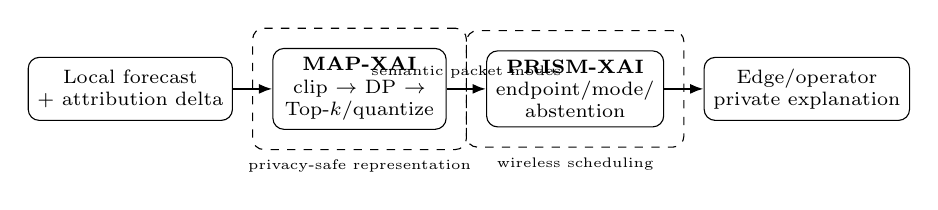
\begin{tikzpicture}[
node distance=4.2mm and 5.0mm,
box/.style={draw,rounded corners,align=center,minimum height=8mm,
minimum width=22mm,font=\scriptsize},
layer/.style={draw,dashed,rounded corners,inner sep=2.5mm},
arr/.style={-{Latex[length=1.7mm]},thick}]
\node[box] (xai) {Local forecast\\+ attribution delta};
\node[box,right=of xai] (map) {\textbf{MAP-XAI}\\clip $\rightarrow$ DP $\rightarrow$\\Top-$k$/quantize};
\node[box,right=of map] (prism) {\textbf{PRISM-XAI}\\endpoint/mode/\\abstention};
\node[box,right=of prism] (op) {Edge/operator\\private explanation};
\draw[arr] (xai)--(map);
\draw[arr] (map)--node[above,font=\tiny]{semantic packet modes}(prism);
\draw[arr] (prism)--(op);
\node[layer,fit=(map),label={[font=\tiny]below:privacy-safe representation}] {};
\node[layer,fit=(prism),label={[font=\tiny]below:wireless scheduling}] {};
\end{tikzpicture}}
\caption{Proposed stack. \mapxai{} determines how a private semantic
explanation is represented; \method{} determines whether, when, and at
what resolution it is delivered.}
\label{fig:stack}
\end{figure}

\subsection{MAP-XAI: private semantic packetization}

Let $t_i^-$ be the last accepted explanation slot. The endpoint forms
$\Delta\bm\phi_{i,t}=\bm\phi_{i,t}-\bm\phi_{i,t_i^-}$ and clips it to
$\ell_2$ radius $C_i$:
\begin{equation}
\overline{\Delta\bm\phi}_{i,t}=
\frac{\Delta\bm\phi_{i,t}}
{\max\{1,\|\Delta\bm\phi_{i,t}\|_2/C_i\}}.
\label{eq:clip}
\end{equation}
For add/remove household adjacency, sensitivity is $\Delta_i=C_i$. A
Gaussian mechanism then releases
\begin{equation}
\widetilde{\Delta\bm\phi}_{i,t}=
\overline{\Delta\bm\phi}_{i,t}+\bm n_{i,t},\quad
\bm n_{i,t}\sim\mathcal N(0,\sigma_{i,t}^2\Delta_i^2\bm I_d).
\label{eq:gauss}
\end{equation}
Only after Eq.~\eqref{eq:gauss} does \mapxai{} retain Top-$k$ coordinates
and quantize their magnitudes. Hence selection and quantization are DP
post-processing. A mode $m=(k,q,\sigma)$ has packet size
\begin{equation}
S_i(m)=S_0+k(\lceil\log_2 d\rceil+q+1),
\label{eq:size}
\end{equation}
where the final bit carries the sign. Different $k$, $q$, and $\sigma$
values define semantic/privacy levels; a no-release action spends no
privacy.

We account for repeated release with R\'enyi-DP (RDP)
~\cite{mironov2017rdp}. At order $\alpha$, a Gaussian release costs
$\rho_{i,t}(\alpha)=\alpha/(2\sigma_{i,t}^2)$. The endpoint composes
these costs and rejects a private release that would exceed the remaining
budget. At the end of the protected horizon,
\begin{equation}
\epsilon_i(\delta_i)=\min_{\alpha}
\left\{\sum_t a_{i,t}\rho_{i,t}(\alpha)+
\frac{\log(1/\delta_i)}{\alpha-1}\right\}.
\label{eq:rdp}
\end{equation}
Privacy is charged when a private packet is exposed outside the trusted
endpoint, even if it later misses the communication deadline. Because
clipping fixes the sensitivity, Eq.~\eqref{eq:gauss} is Gaussian DP at
each release; Top-$k$ selection, quantization, and packet reconstruction
are post-processing. RDP composition in Eq.~\eqref{eq:rdp} therefore
provides the stated user-level horizon guarantee whenever every admitted
release remains inside the tracked RDP budget.

\paragraph{Content-privacy guarantee.}
Under the add/remove household adjacency above, each exposed noisy delta
has order-$\alpha$ RDP cost $\rho_{i,t}(\alpha)=\alpha/(2\sigma_{i,t}^2)$.
Adaptive RDP composition is additive, so every packet-content transcript
admitted by Eq.~\eqref{eq:rdp} is $(\epsilon_i(\delta_i),\delta_i)$-DP.
Top-$k$ selection, quantization, reconstruction, and controller operations
that depend only on public state and previously released private outputs
are post-processing. This guarantee is for released content; an independent
timing side channel remains outside the threat model stated above.

\subsection{PRISM-XAI: privacy-accounted scheduling}

Let $A_{i,t}$ be AoX and $w^{\rm crit}_{i,t}\geq 1$ a public
criticality weight. A candidate mode must fit the available resource
blocks, meet the $D_i^{\max}$ deadline, and pass RDP admission. The
controller estimates $G_{i,t}(m)$, the expected reduction in explanation
loss, from AoX, public criticality, channel state, mode resolution,
remaining budget, and previously released privatized residual evidence;
it never uses the non-private oracle online. Unsent residual evidence is
accumulated and decayed, so a private release is considered only when the
predicted semantic signal is large enough relative to the DP-noise floor.

For a feasible mode, define gain per transmitted bit
\begin{equation}
\Gamma_{i,t}(m)=\frac{G_{i,t}(m)}{S_i(m)}.
\label{eq:gainbit}
\end{equation}
The nonzero candidate set includes a \mapxai{} packet mode, optional
higher-resolution modes, and a coarse zonal mode; zero transmission is
always available. A richer mode replaces the \mapxai{} mode only when
its gain per bit exceeds the \mapxai{} value by a configured margin. The
slot utility also rewards criticality-weighted AoX and under-served
endpoints while penalizing energy and RDP shadow price. The resulting
multiple-choice knapsack selects at most one mode per endpoint under the
slot resource-block limit. A minimum critical-event coverage target and
minimum Jain fairness are included as service guardrails. This structure
makes \mapxai{} the privacy-valid semantic layer and \method{} the
resource-allocation layer above it. With $M$ candidate modes per endpoint
and $B$ available resource blocks, the slot-level multiple-choice knapsack
can be solved by dynamic programming in $O(NMB)$ time; in our experiments
$M$ and $B$ are small constants. The online decision therefore does not
require re-running the forecaster or a non-private explanation oracle at
the edge.

\section{Evaluation}

\subsection{Data, wireless setting, and baselines}

We use Open Power System Data (OPSD) household data and UCI
ElectricityLoadDiagrams20112014~\cite{opsd2020household,uci2015eld}.
Nine OPSD endpoints are grouped into three synthetic zones and 32 UCI
endpoints into four synthetic zones. Each forecaster uses 12 lag,
rolling-statistic, and calendar features. The tree model obtains
RMSE/MAE $0.926/0.545$ on OPSD and $1.289/0.221$ on UCI. We evaluate two
attribution implementations, TreeSHAP and feature ablation, to ensure the
scheduler conclusions are not tied to one tree explainer.

The uplink abstraction uses eight 180~kHz resource blocks, 1~ms slots,
5~ms deadlines, 3.5~GHz carrier frequency, path loss, correlated
shadowing, small-scale fading, edge delay, and bursty failures inspired
by 3GPP TR~38.901~\cite{3gpp38901}. It is a reproducible
scheduler-level stress trace, not a link-level field validation.

The main selective-release matrix uses $512$ evaluation slots after $96$
calibration slots, privacy budgets $\epsilon_{\max}\in\{8,16,32\}$ with
$\delta=10^{-5}$, at most eight private releases per endpoint, a 5\%
minimum critical-event coverage target, and 0.88 minimum Jain fairness.
There are $2$ datasets $\times$ $2$ XAI methods $\times$ $3$ privacy
budgets $\times$ $6$ schedulers $\times$ $10$ paired seeds $=720$ runs.

External baselines are periodic fixed-DP, channel-aware fixed-DP,
AoX-aware fixed-DP, and joint scheduling with full, uncompressed private
packets. We additionally report \emph{MAP-XAI-only}, which is not an
external baseline: it restricts our stack to the \mapxai{} packet mode
and therefore isolates the incremental effect of full PRISM scheduling.
Metrics include transmitted traffic, Top-$K$ and cosine agreement,
critical-event coverage and recall, intervention precision, false
intervention, bits per correct intervention, deadline misses, Jain
fairness, and spent privacy.

\subsection{Feasibility diagnostics}

A separate three-seed feasibility ladder at $\epsilon_{\max}=4$ removes
one transformation at a time: (A) oracle explanation, (B) clipping only,
(C) clipping plus cumulative Gaussian DP with a full packet, and (D) DP
plus semantic compression. A release sweep then varies
$\epsilon\in\{2,4,8,16,32\}$ and the maximum private releases per
endpoint $M\in\{4,8,16,32,64\}$. These diagnostics are not used to tune
the reported 720-run matrix; they identify the mechanism that limits
explanation utility.

\section{Results}

\subsection{Communication efficiency and operational trade-off}

Table~\ref{tab:main} macro-averages the 12 dataset/XAI/privacy settings.
The proposed stack operates at a deliberately selective point: mean
critical-event coverage is 7.8\%, versus 24.8\% for joint full-packet
scheduling and 87.5\% for AoX fixed-DP. The traffic reduction must
therefore be read jointly with coverage, precision, and bits per correct
intervention rather than as a free throughput gain.

\begin{table*}[t]
\caption{Macro-average over 12 dataset/XAI/privacy settings (10 paired
seeds each). \mapxai{}-only is a proposed-component ablation, not an
external baseline. Lower traffic and kbit/correct are better; higher
Top-$K$, coverage, recall, precision, and fairness are better.}
\label{tab:main}
\centering
\footnotesize
\setlength{\tabcolsep}{4.1pt}
\begin{tabular}{lccccccc}
\toprule
Method & Traffic (kbit) & Top-$K$ & Crit. cov. & Crit. recall & Precision & kbit/correct & Fairness \\
\midrule
Periodic fixed-DP & 4645.2 & 0.252 & 0.383 & 0.178 & 0.226 & 707.0 & 1.000 \\
Channel fixed-DP & 4573.8 & 0.264 & 0.334 & 0.161 & 0.189 & 1146.6 & 0.737 \\
AoX fixed-DP & 4643.6 & 0.255 & 0.875 & 0.386 & 0.285 & 23.6 & 0.999 \\
Joint full packet & 1655.4 & 0.260 & 0.248 & 0.117 & 0.314 & 25.5 & 0.965 \\
\midrule
\mapxai{}-only (ours) & 243.7 & 0.265 & 0.078 & 0.037 & \textbf{0.538} & \textbf{10.0} & 0.991 \\
\method{} (ours) & \textbf{242.5} & \textbf{0.279} & 0.078 & 0.037 & 0.510 & \textbf{10.0} & 0.991 \\
\bottomrule
\end{tabular}
\end{table*}

\begin{figure*}[t]
\centering
\begin{minipage}{0.49\textwidth}
\centering
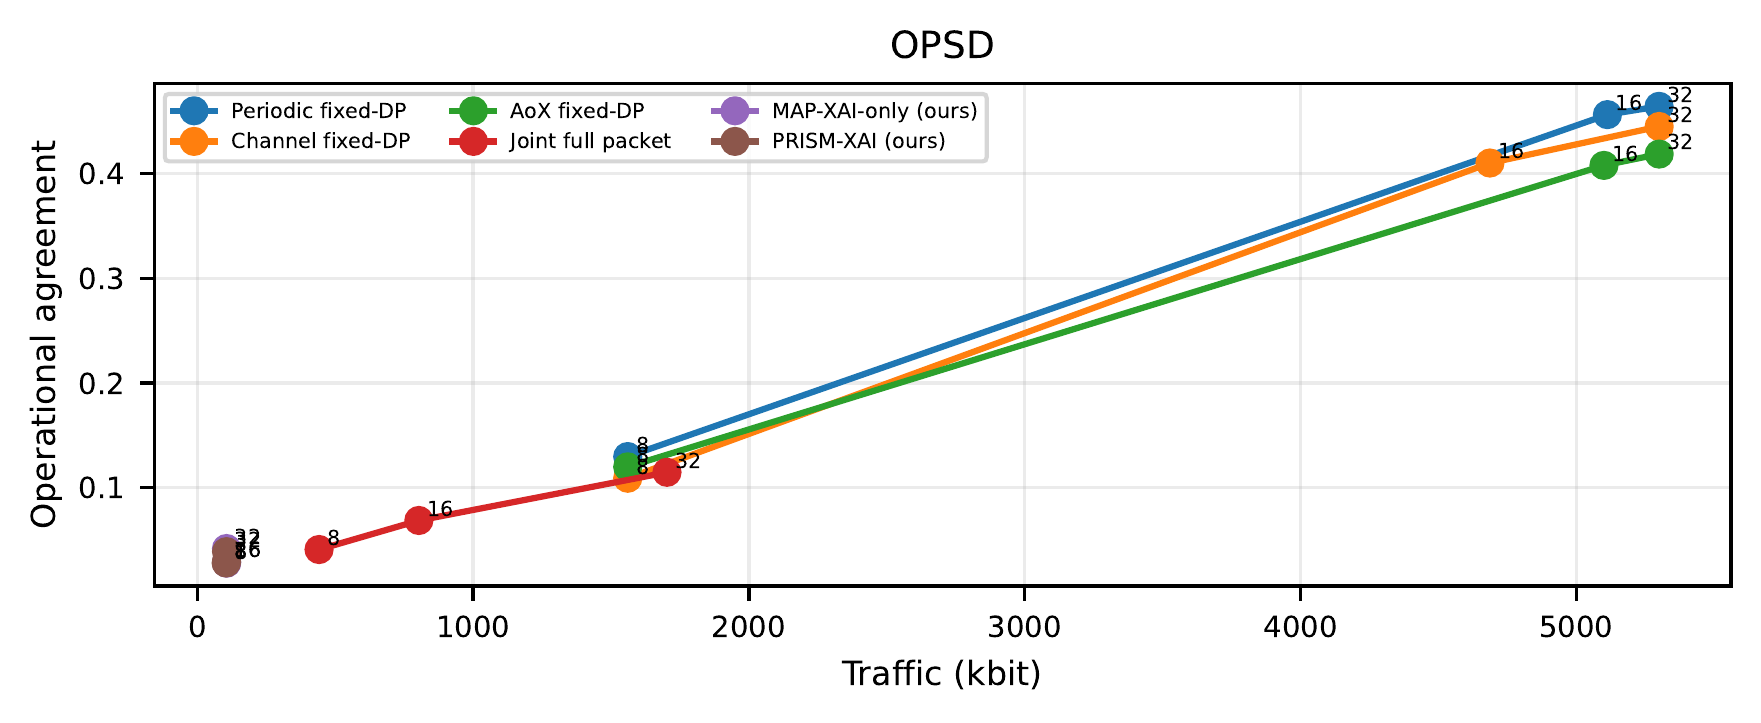
\includegraphics[width=\linewidth]{v19_pareto_main_opsd.png}\\[-1mm]
{\scriptsize (a) OPSD: communication--operation}
\end{minipage}\hfill
\begin{minipage}{0.49\textwidth}
\centering
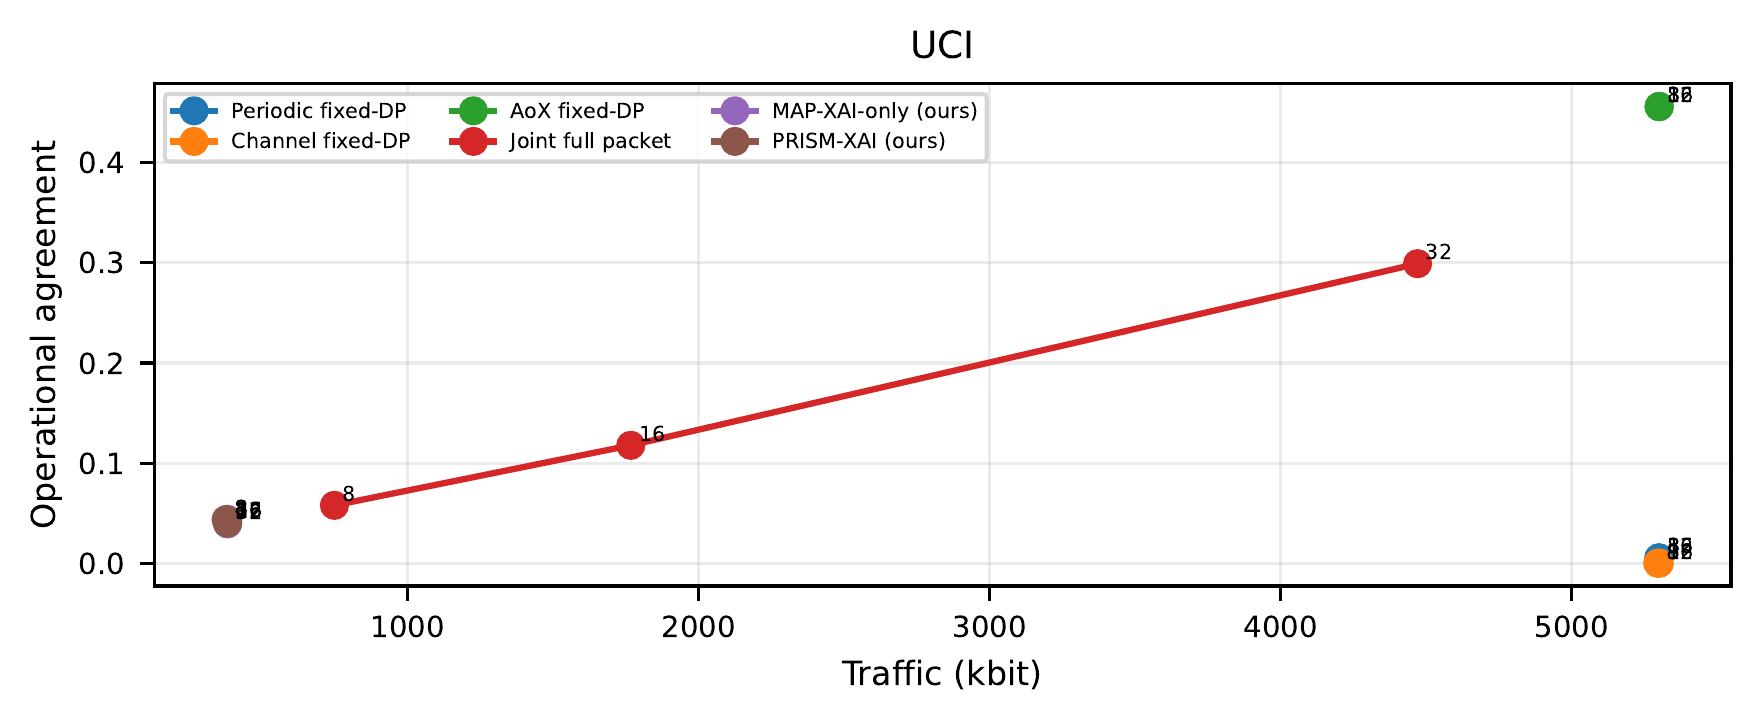
\includegraphics[width=\linewidth]{v19_pareto_main_uci.png}\\[-1mm]
{\scriptsize (b) UCI: communication--operation}
\end{minipage}\\[-1mm]
\begin{minipage}{0.49\textwidth}
\centering
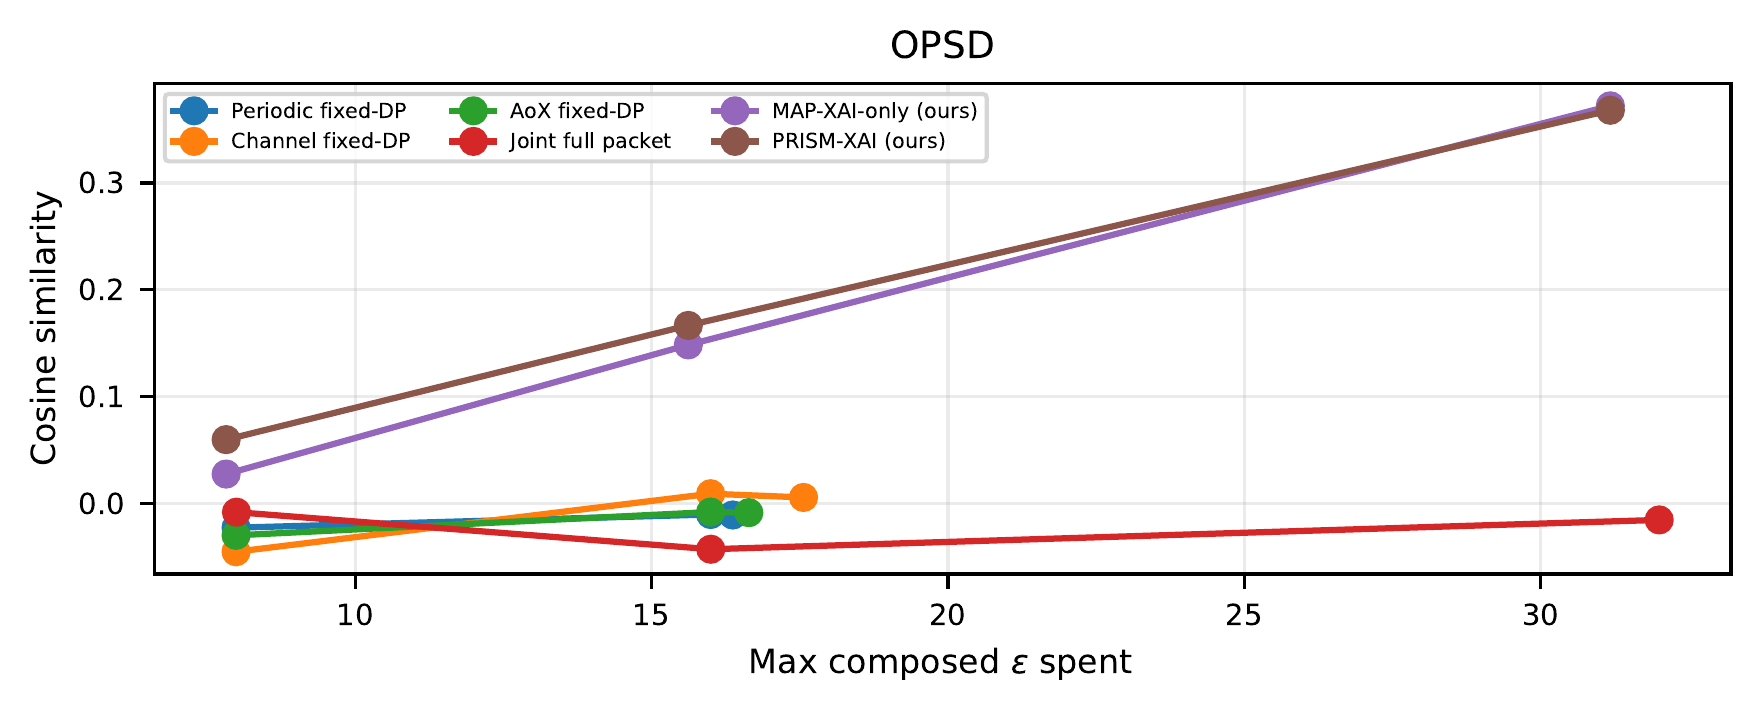
\includegraphics[width=\linewidth]{v19_privacy_main_opsd.png}\\[-1mm]
{\scriptsize (c) OPSD: privacy--fidelity}
\end{minipage}\hfill
\begin{minipage}{0.49\textwidth}
\centering
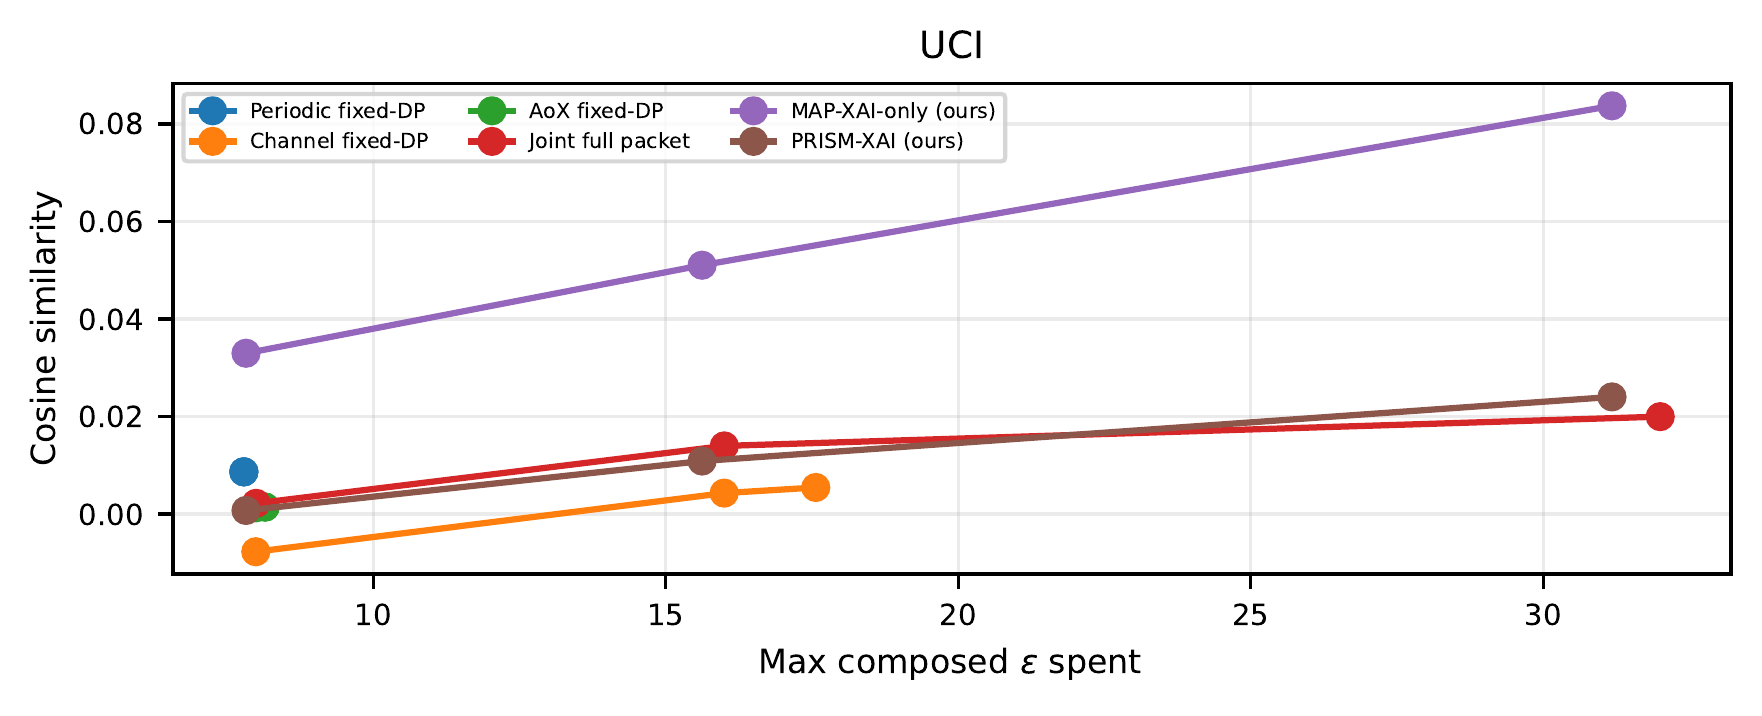
\includegraphics[width=\linewidth]{v19_privacy_main_uci.png}\\[-1mm]
{\scriptsize (d) UCI: privacy--fidelity}
\end{minipage}\\[-1mm]
\begin{minipage}{0.49\textwidth}
\centering
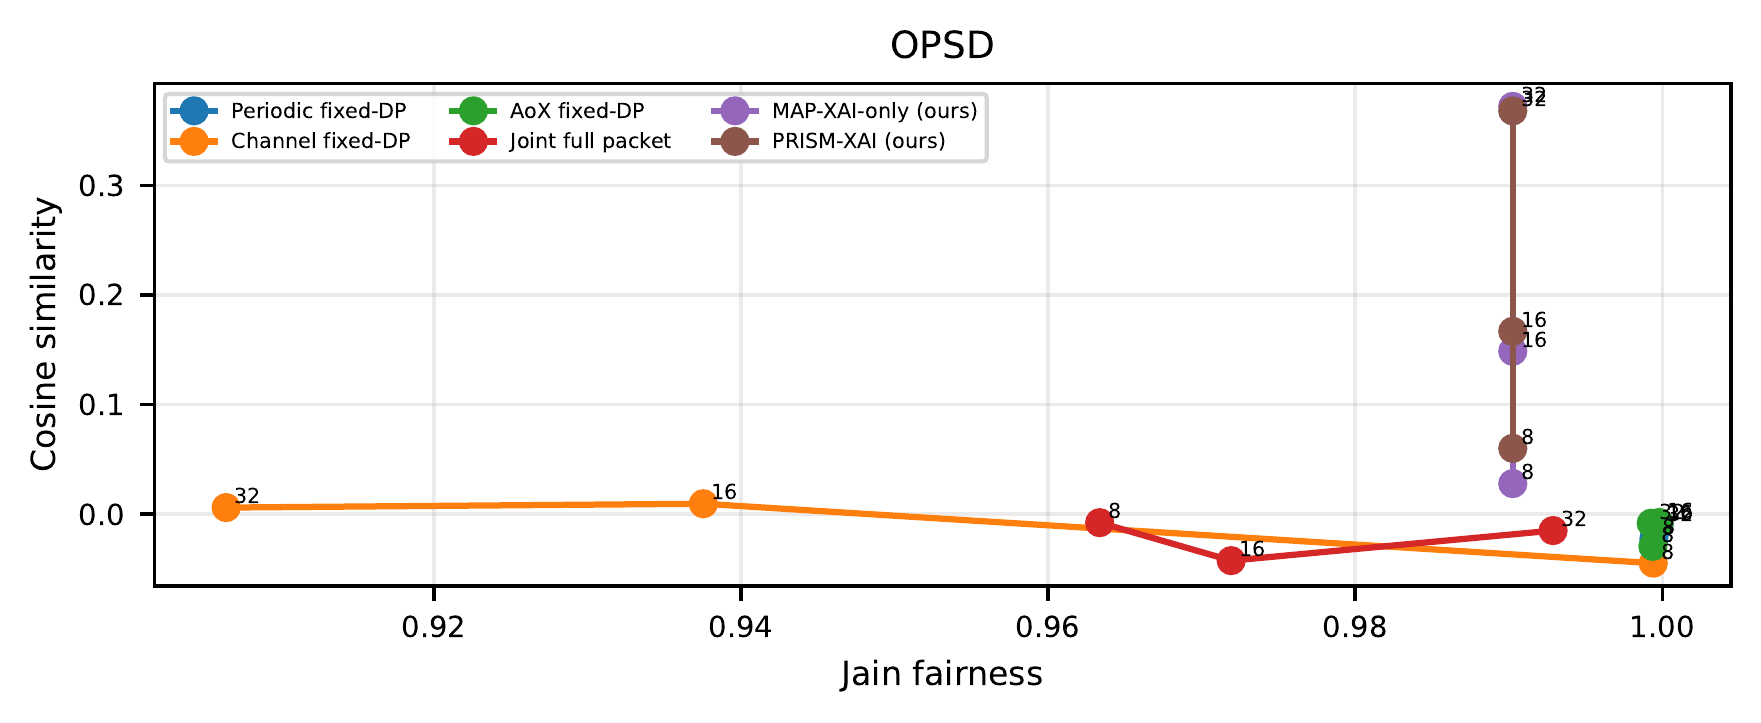
\includegraphics[width=\linewidth]{v19_fairness_main_opsd.png}\\[-1mm]
{\scriptsize (e) OPSD: fairness--fidelity}
\end{minipage}\hfill
\begin{minipage}{0.49\textwidth}
\centering
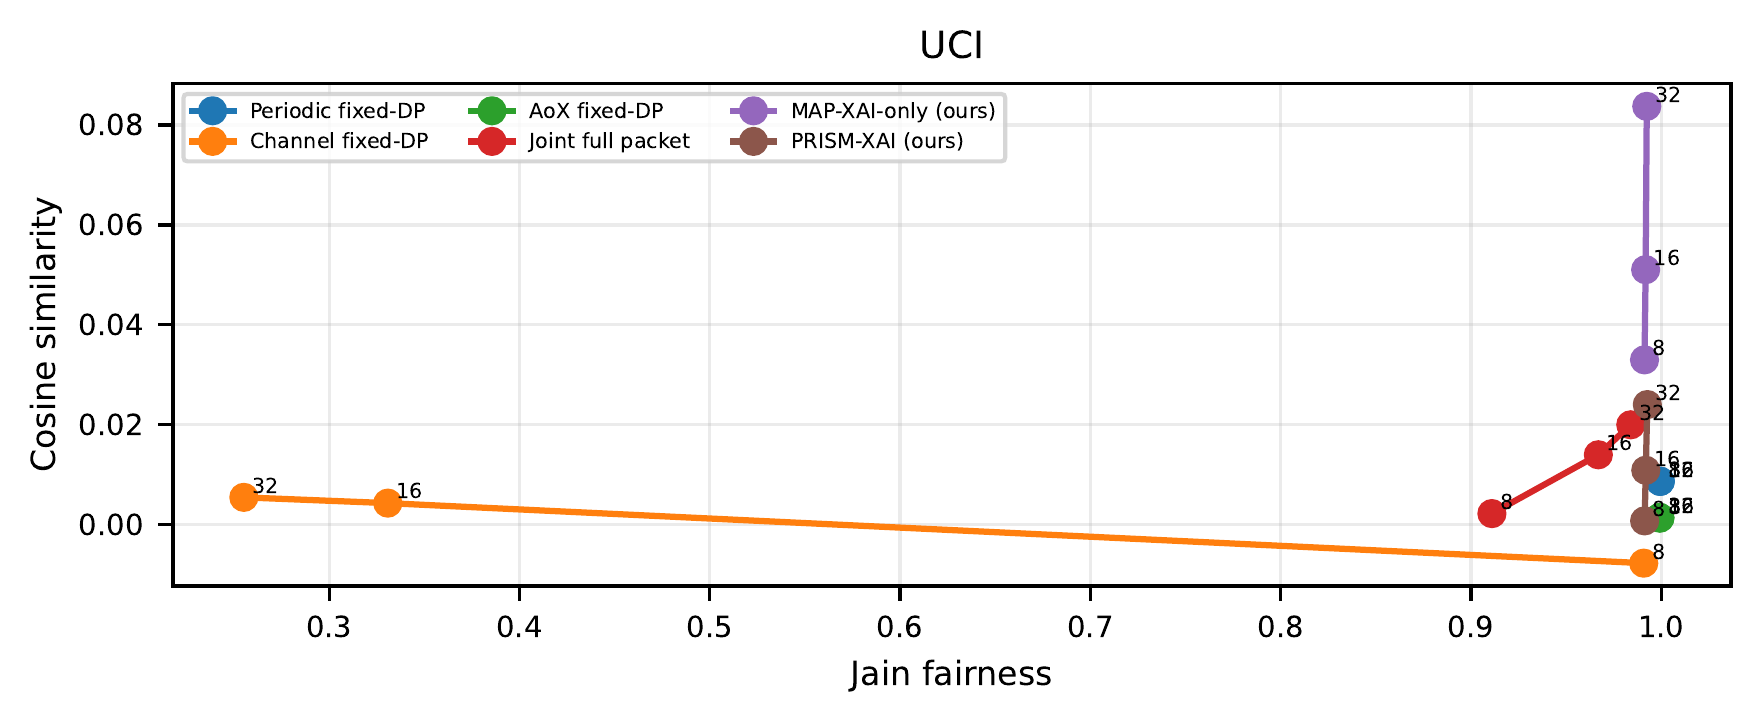
\includegraphics[width=\linewidth]{v19_fairness_main_uci.png}\\[-1mm]
{\scriptsize (f) UCI: fairness--fidelity}
\end{minipage}
\caption{\textbf{Main v19 evidence.} Rows show communication--operation,
privacy--fidelity, and fairness--fidelity trade-offs. Curves average both XAI
implementations and 10 paired seeds at $\epsilon_{\max}\in\{8,16,32\}$.
MAP-XAI-only is our restricted packetization layer, not an external baseline.
The proposed stack occupies a low-traffic, high-fairness selective-release
region; higher external-baseline coverage requires substantially more traffic.}
\label{fig:mainv19}
\end{figure*}

Figure~\ref{fig:mainv19} is the primary v19 result. Averaged
condition-by-condition, PRISM transmits 94.6\% less explanation traffic than
the three fixed-DP schedulers and 79.4\% less than joint full-packet
scheduling. Paired 95\% confidence intervals show lower traffic in all 48
external-baseline comparisons and lower bits per correct intervention in
45/48. Top-$K$ is statistically tied in 37/48 comparisons, higher in eight,
and lower in three; intervention precision is higher in 38/48. The result is
therefore an efficiency claim rather than universal recall dominance: AoX
fixed-DP serves many more critical events by transmitting much more often.

MAP-XAI-only isolates our packetization contribution. Relative to it, full
PRISM has statistically tied critical-event recall, coverage, and fairness in
all 12 dataset/XAI/privacy settings; traffic is lower in five and tied in
seven, while Top-$K$ is tied in 11 and higher in one. Across all 120 PRISM
runs there are no privacy-budget violations; the minimum critical-event
coverage is 5.98\% and minimum Jain fairness is 0.972, above the configured
5\% and 0.88 guardrails.

\begin{table}[t]
\caption{Representative $\epsilon_{\max}=8$ results, averaged over the
two attribution methods and 10 paired seeds. MAP is the proposed
MAP-XAI-only restriction.}
\label{tab:eps8}
\centering
\scriptsize
\setlength{\tabcolsep}{2.4pt}
\resizebox{\columnwidth}{!}{%
\begin{tabular}{llccccc}
\toprule
Data & Method & Traffic (kbit) & Crit. cov. & Crit. recall & Precision & kbit/correct \\
\midrule
OPSD & AoX fixed-DP & 1560.6 & 0.279 & 0.120 & 0.202 & 34.9 \\
     & Joint full & 441.4 & 0.084 & 0.041 & 0.267 & 32.1 \\
     & MAP-XAI-only & 106.2 & 0.071 & 0.028 & 0.303 & 9.9 \\
     & PRISM-XAI & \textbf{104.6} & 0.071 & 0.028 & \textbf{0.306} & \textbf{9.7} \\
\midrule
UCI & AoX fixed-DP & 5300.2 & 0.997 & 0.456 & 0.362 & 14.1 \\
    & Joint full & 748.4 & 0.130 & 0.058 & 0.398 & 16.2 \\
    & MAP-XAI-only & 381.4 & 0.090 & 0.044 & 0.488 & 10.9 \\
    & PRISM-XAI & \textbf{376.2} & 0.090 & 0.044 & \textbf{0.493} & \textbf{10.7} \\
\bottomrule
\end{tabular}}
\end{table}

Table~\ref{tab:eps8} exposes the representative $\epsilon_{\max}=8$
operating point without dataset-level macro-averaging. The communication
savings persist on both OPSD and UCI, while the much higher AoX-DP
coverage remains explicit. This prevents the aggregate result from
masking the central service trade-off: the proposed stack is designed
for selective, high-value explanation delivery rather than exhaustive
critical-event service.

\begin{figure*}[t]
\centering
\setlength{\tabcolsep}{1pt}
\begin{tabular}{cc}
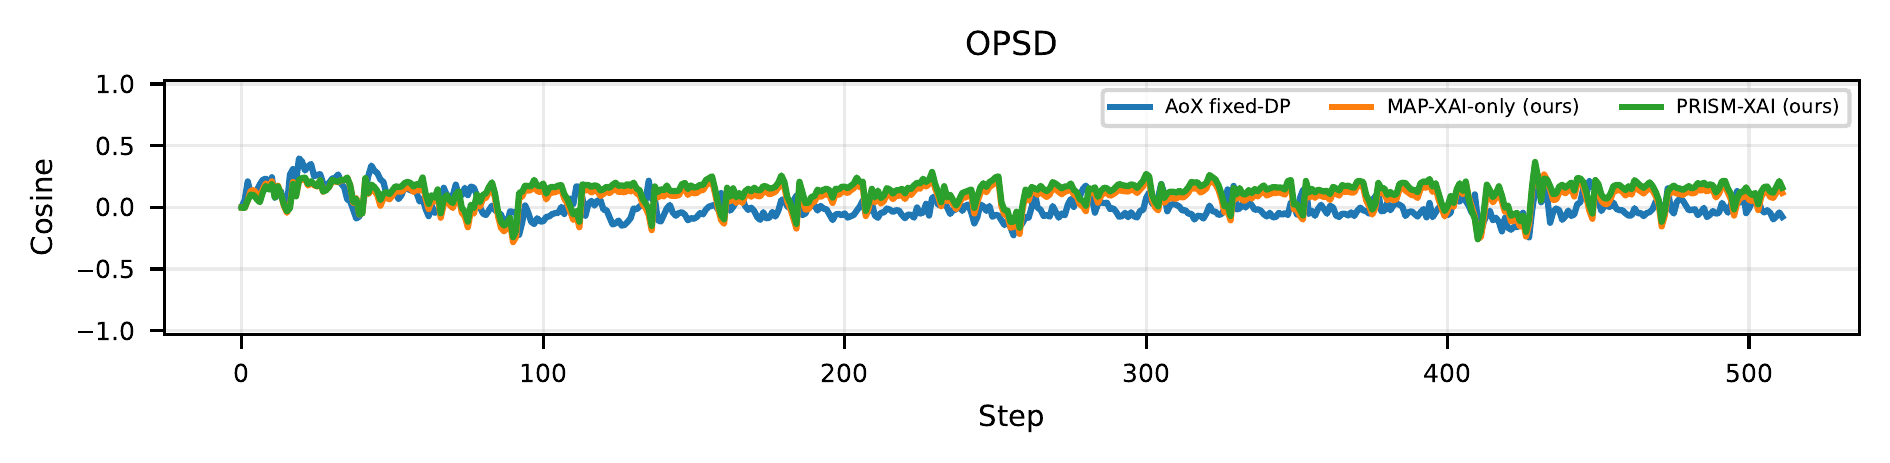
\includegraphics[width=0.485\textwidth]{regime_main_cosine_opsd.png} &
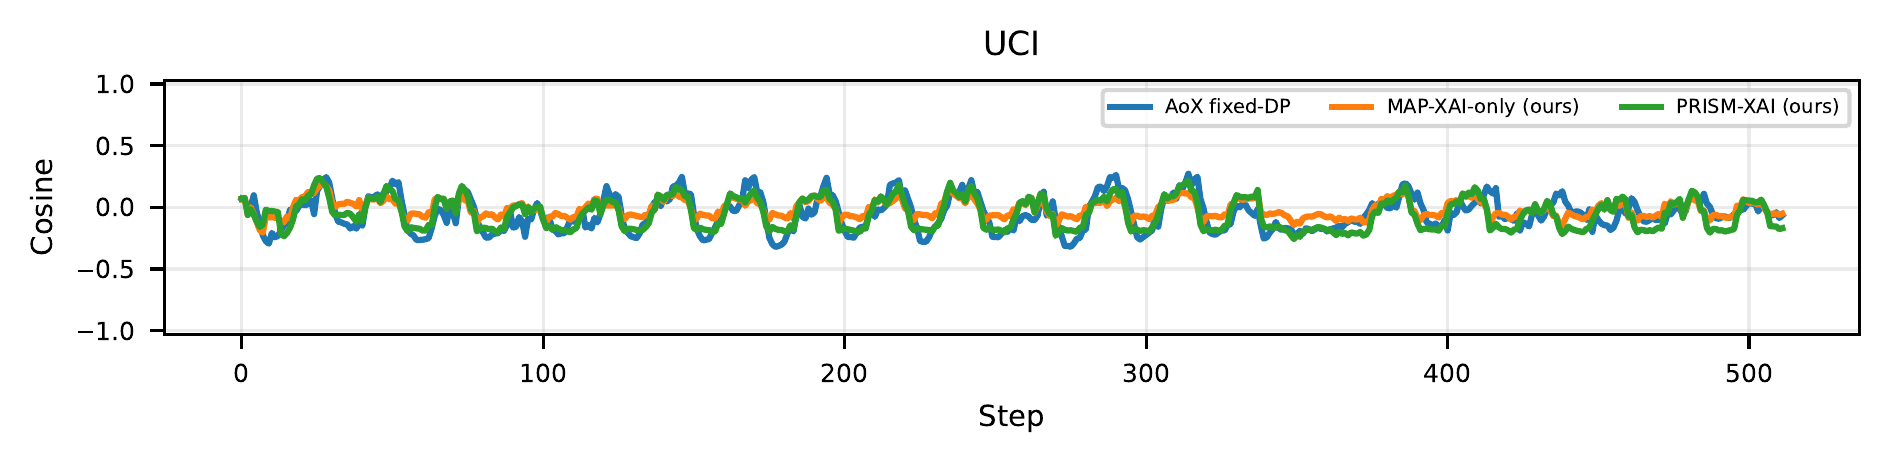
\includegraphics[width=0.485\textwidth]{regime_main_cosine_uci.png}\\[-1mm]
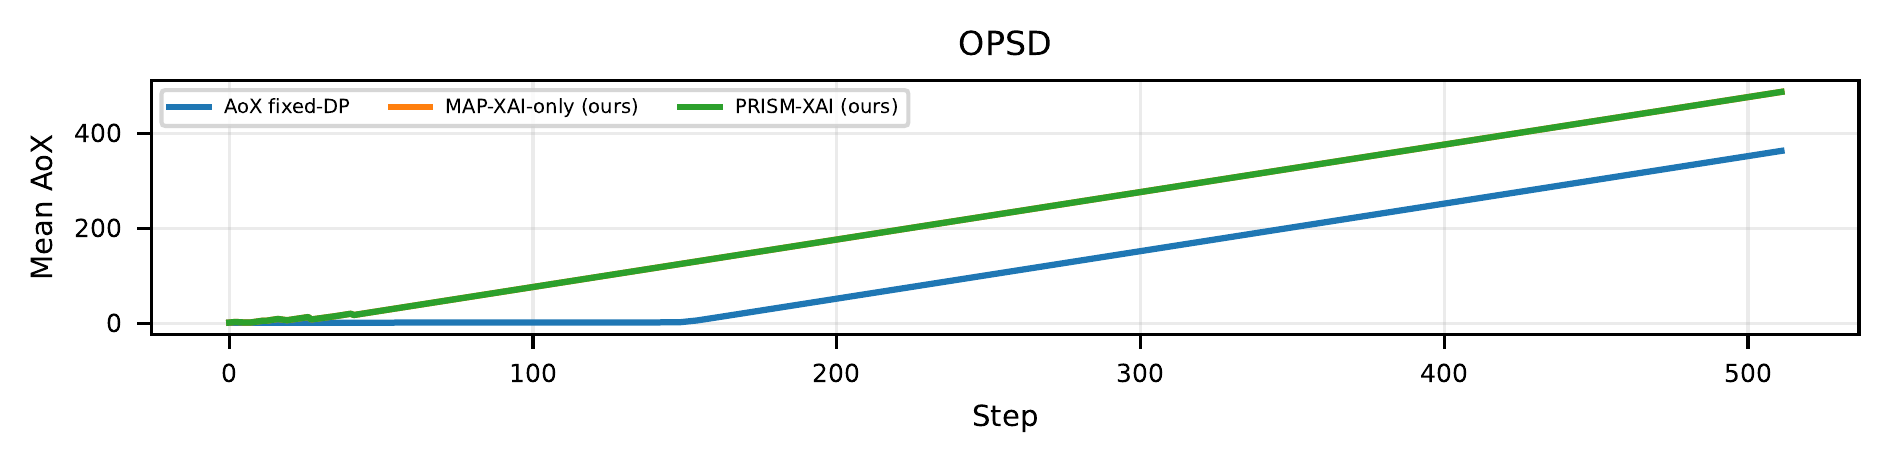
\includegraphics[width=0.485\textwidth]{regime_main_aox_opsd.png} &
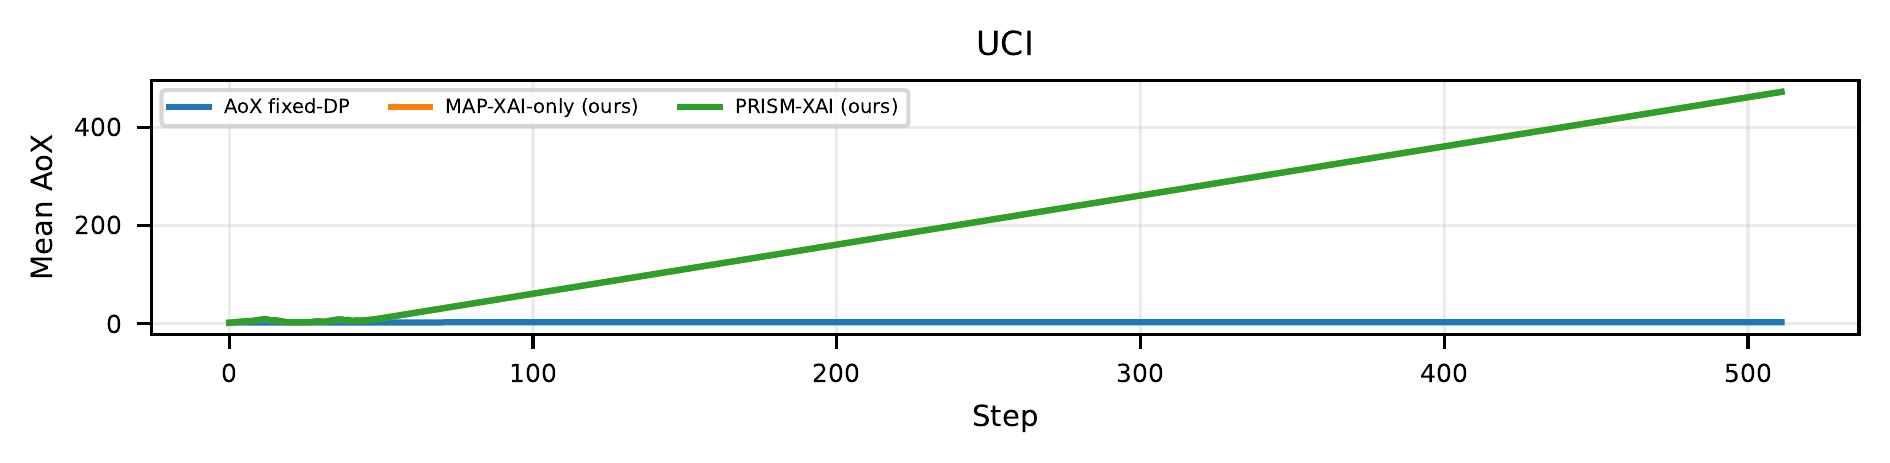
\includegraphics[width=0.485\textwidth]{regime_main_aox_uci.png}\\[-1mm]
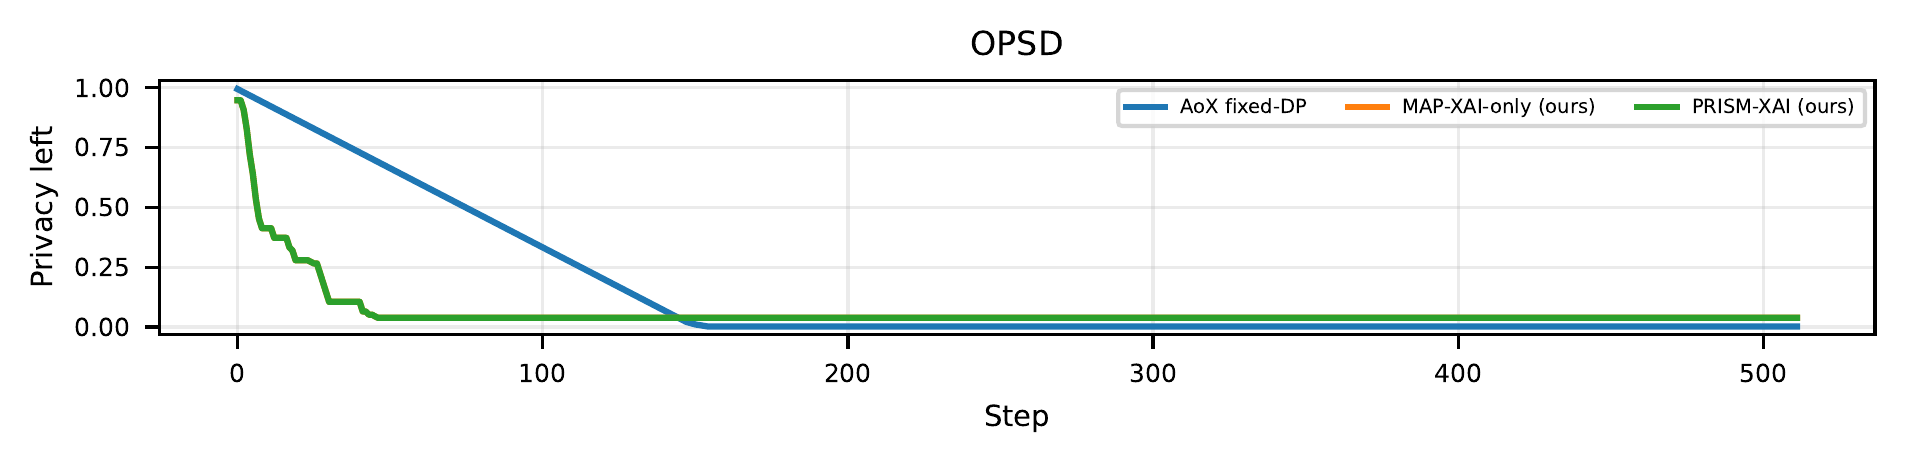
\includegraphics[width=0.485\textwidth]{regime_main_privacy_opsd.png} &
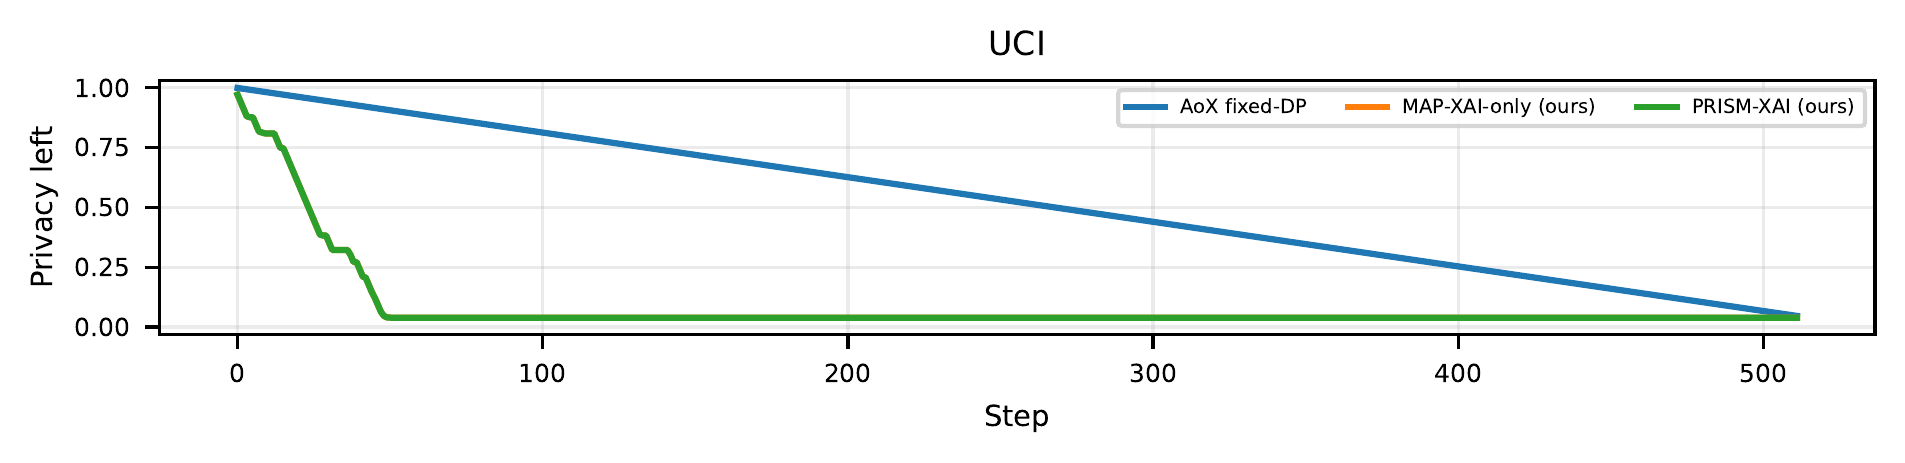
\includegraphics[width=0.485\textwidth]{regime_main_privacy_uci.png}\\[-1mm]
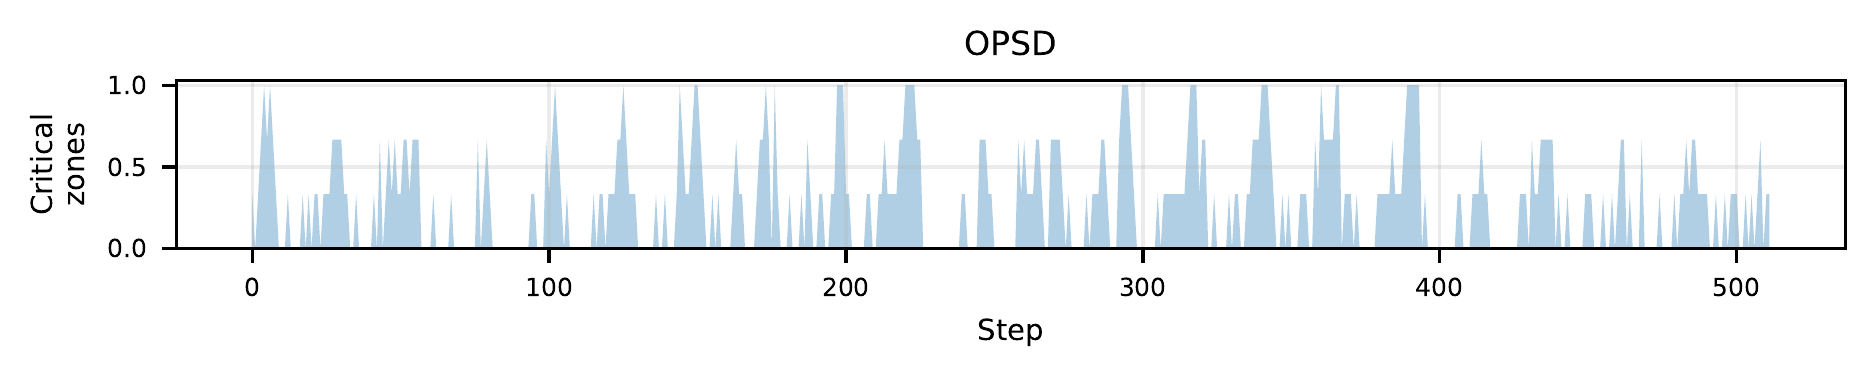
\includegraphics[width=0.485\textwidth]{regime_main_critical_opsd.png} &
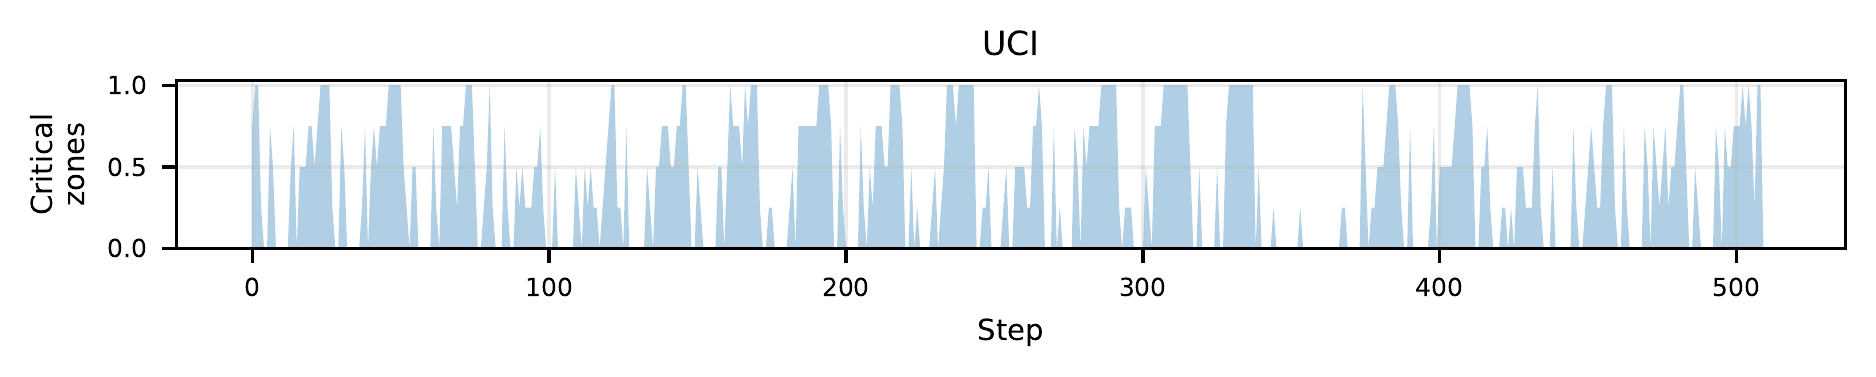
\includegraphics[width=0.485\textwidth]{regime_main_critical_uci.png}
\end{tabular}
\caption{\textbf{Main v19 regime evidence} at $\epsilon_{\max}=8$, seed 11,
averaged over the two XAI implementations. Rows show explanation cosine,
mean AoX, remaining privacy fraction, and the public critical-zone process.
MAP-XAI-only and PRISM exhaust their deliberately small private-release
allowance early and then accumulate AoX; AoX fixed-DP continues releasing and
therefore keeps AoX lower at much larger communication cost.}
\label{fig:regime}
\end{figure*}

\begin{table}[t]
\caption{Paired 95\% CI outcomes across matched settings. ``Better''
means the PRISM-minus-reference confidence interval is strictly favorable;
``tie'' contains zero. MAP-XAI-only is an internal ablation.}
\label{tab:paired}
\centering
\scriptsize
\setlength{\tabcolsep}{3.0pt}
\begin{tabular}{lcccc}
\toprule
Reference & $n$ & Traffic lower & kbit/correct lower & Top-$K$: B/T/W \\
\midrule
Fixed-DP schedulers & 36 & 36 & 34 & 6/27/3 \\
Joint full packet & 12 & 12 & 11 & 2/9/1 \\
MAP-XAI-only (ours) & 12 & 5 & 0 & 1/11/0 \\
\bottomrule
\end{tabular}
\end{table}

Figure~\ref{fig:regime} supplies the temporal evidence behind the aggregate results: selective private modes spend their finite release allowance early and then accumulate AoX, whereas AoX fixed-DP continues transmitting. Table~\ref{tab:paired} separates statistical robustness from raw means.
Against the external baselines, traffic is lower in every paired setting,
and Top-$K$ is usually indistinguishable or better. Against the internal
MAP-XAI-only restriction, the intended result is compatibility rather
than dominance: coverage, recall, and fairness are tied in all 12
settings while the full controller retains access to additional modes.

\subsection{Where explanation fidelity is lost}

Figure~\ref{fig:ladder} gives the central diagnostic result. Clipping is
almost lossless: Top-$K$ changes from 1.000 to 0.990 on OPSD and 0.993 on
UCI. The large collapse occurs when cumulative Gaussian DP is added:
Top-$K$ becomes 0.241 and 0.282, respectively, close to the random
Top-$K$ reference of 0.25. Applying Top-$k$/quantization after DP changes
these values only to 0.252 and 0.295. Hence semantic compression is not
the main cause of the observed fidelity limit. Once privacy noise has
removed the signal, a wireless scheduler cannot reconstruct it.

\begin{figure*}[t]
\centering
\begin{minipage}{0.49\textwidth}
\centering
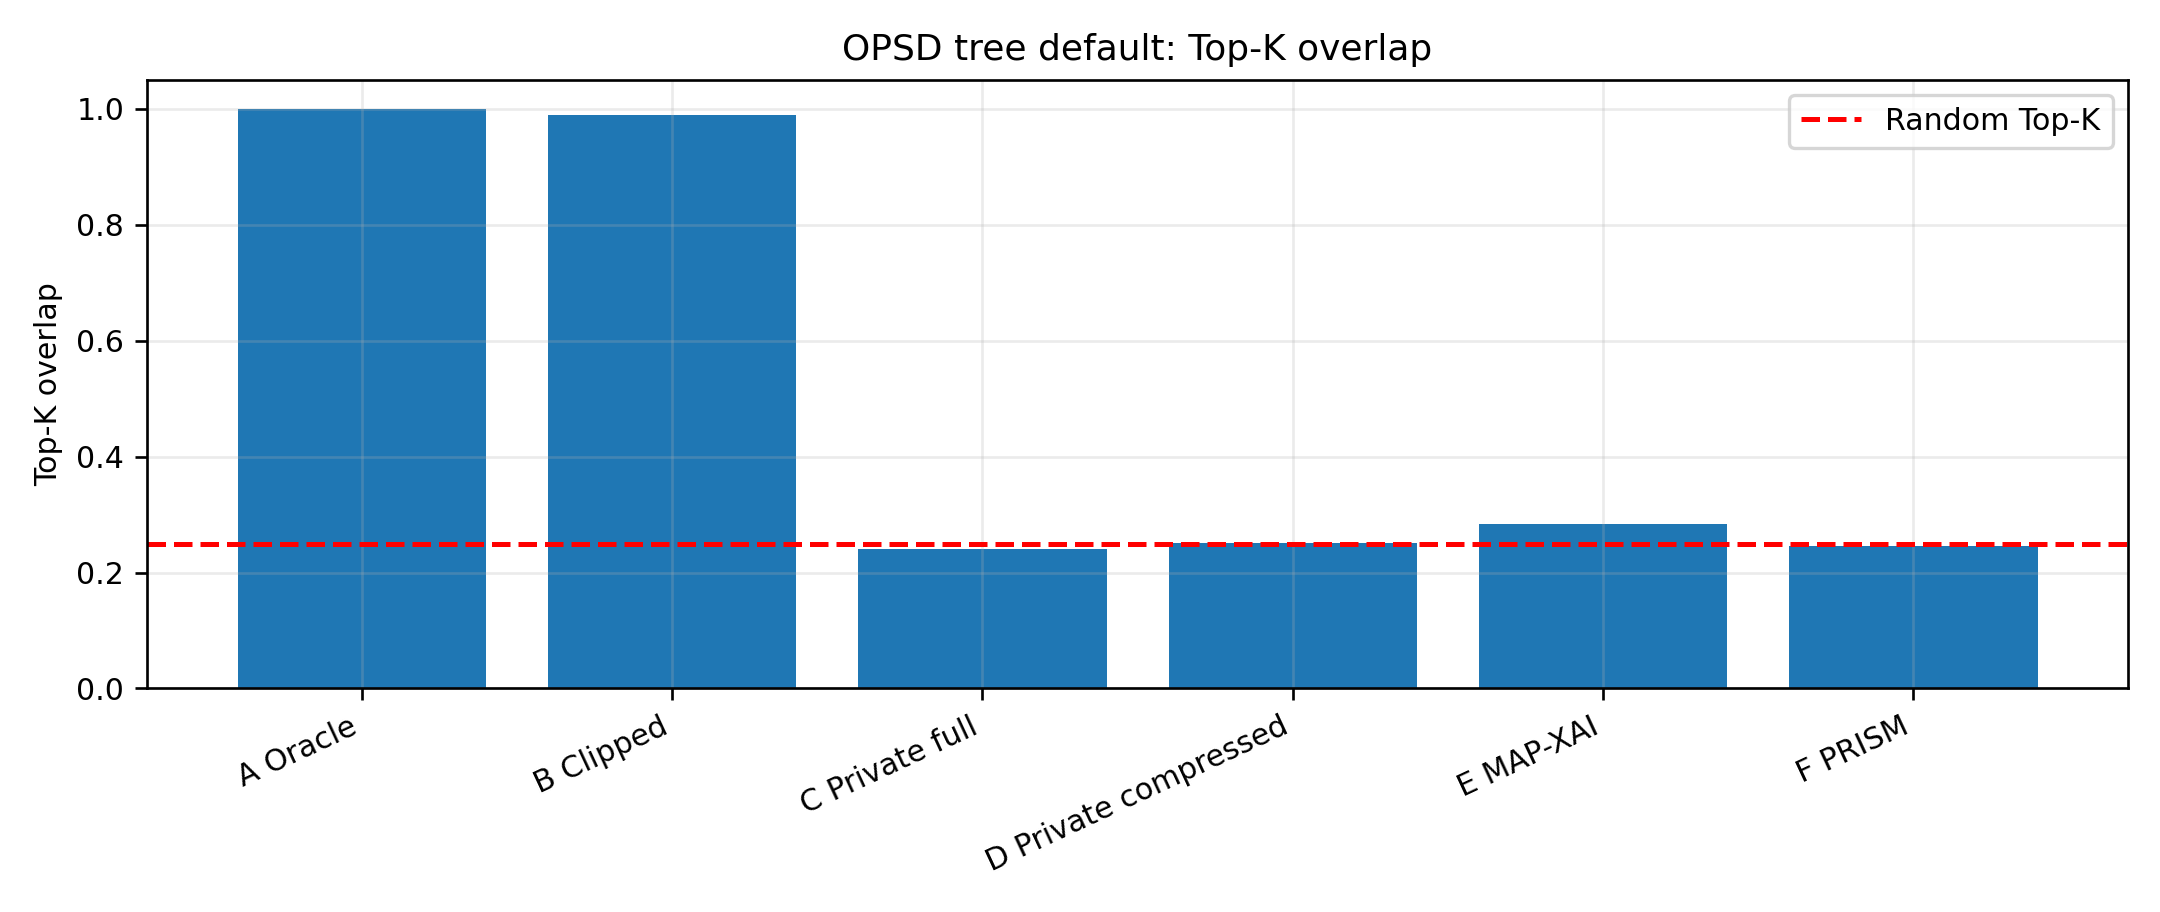
\includegraphics[width=\linewidth]{opsd_tree_default_ladder_topk.png}\\[-1mm]
{\scriptsize (a) OPSD}
\end{minipage}\hfill
\begin{minipage}{0.49\textwidth}
\centering
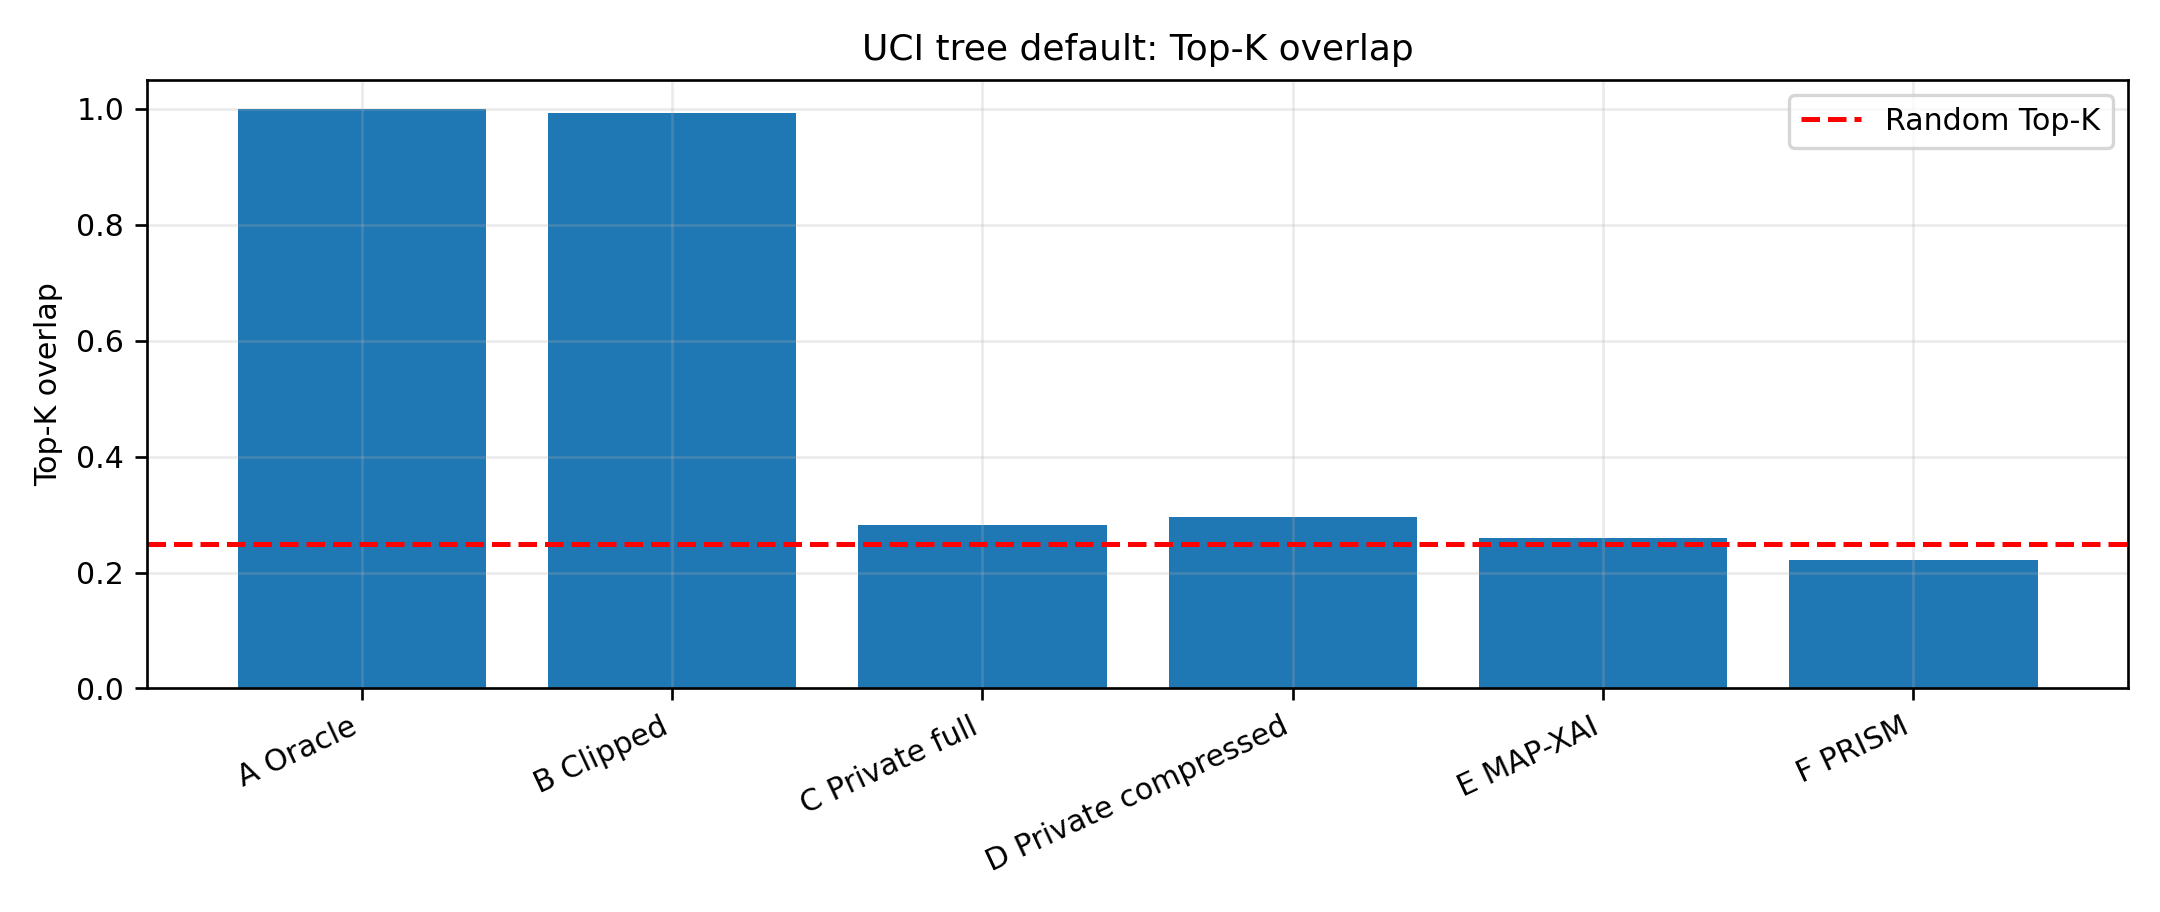
\includegraphics[width=\linewidth]{uci_tree_default_ladder_topk.png}\\[-1mm]
{\scriptsize (b) UCI}
\end{minipage}
\caption{Feasibility ladder at $\epsilon_{\max}=4$. Clipping preserves
Top-$K$ almost perfectly; the dominant collapse occurs when cumulative
household-level DP is introduced. The scheduler stages are shown only to
complete the mechanism ladder, not as an external PRISM-versus-MAP contest.}
\label{fig:ladder}
\end{figure*}

The privacy--release sweep confirms why selective release is useful.
At $\epsilon=32$, UCI Top-$K$ is 0.488 with $M=4$ private releases but
falls toward 0.284 at $M=64$ while coverage grows from 10.3\% to 53.5\%.
On OPSD, $M=16$ gives Top-$K$ 0.375 at 31.1\% coverage, whereas $M=64$
gives Top-$K$ 0.287 at 83.0\% coverage. Figure~\ref{fig:frontier} shows
this feasibility boundary. Higher coverage is possible, but spending a
fixed household privacy budget over more releases increases the noise per
release and can reduce explanation fidelity. This is the reason for the
M8 selective-release operating point in the main experiment.

\begin{figure*}[t]
\centering
\begin{minipage}{0.49\textwidth}
\centering
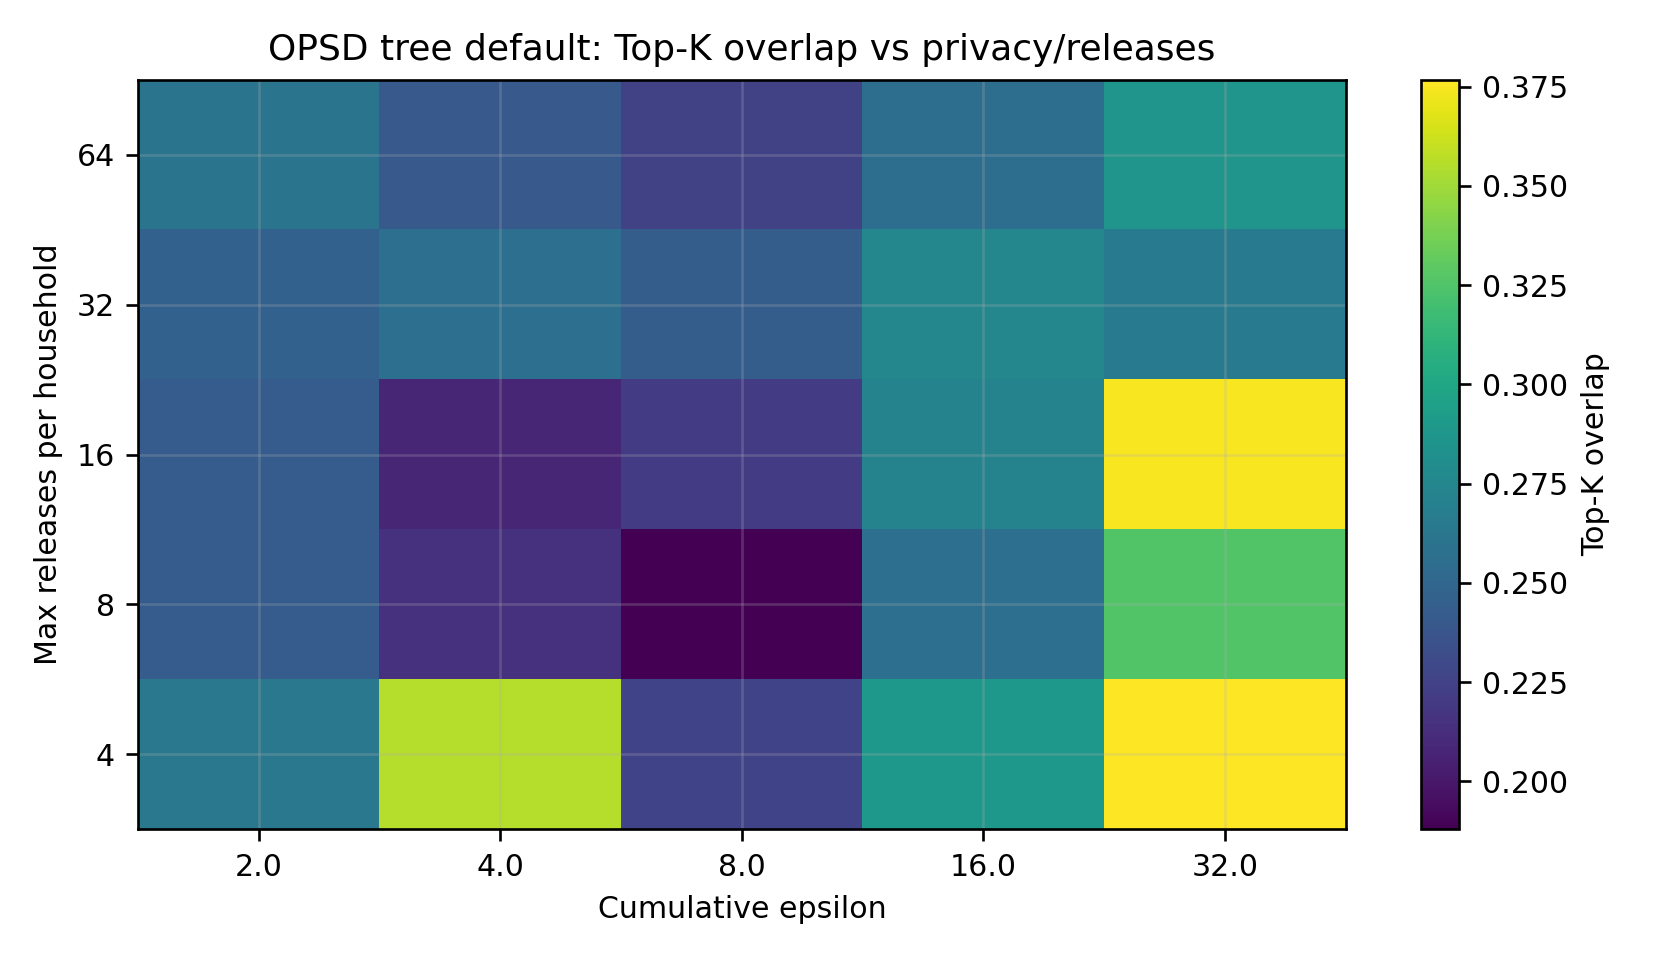
\includegraphics[width=\linewidth]{opsd_tree_default_privacy_sweep_topk_overlap.png}\\[-1mm]
{\scriptsize (a) OPSD}
\end{minipage}\hfill
\begin{minipage}{0.49\textwidth}
\centering
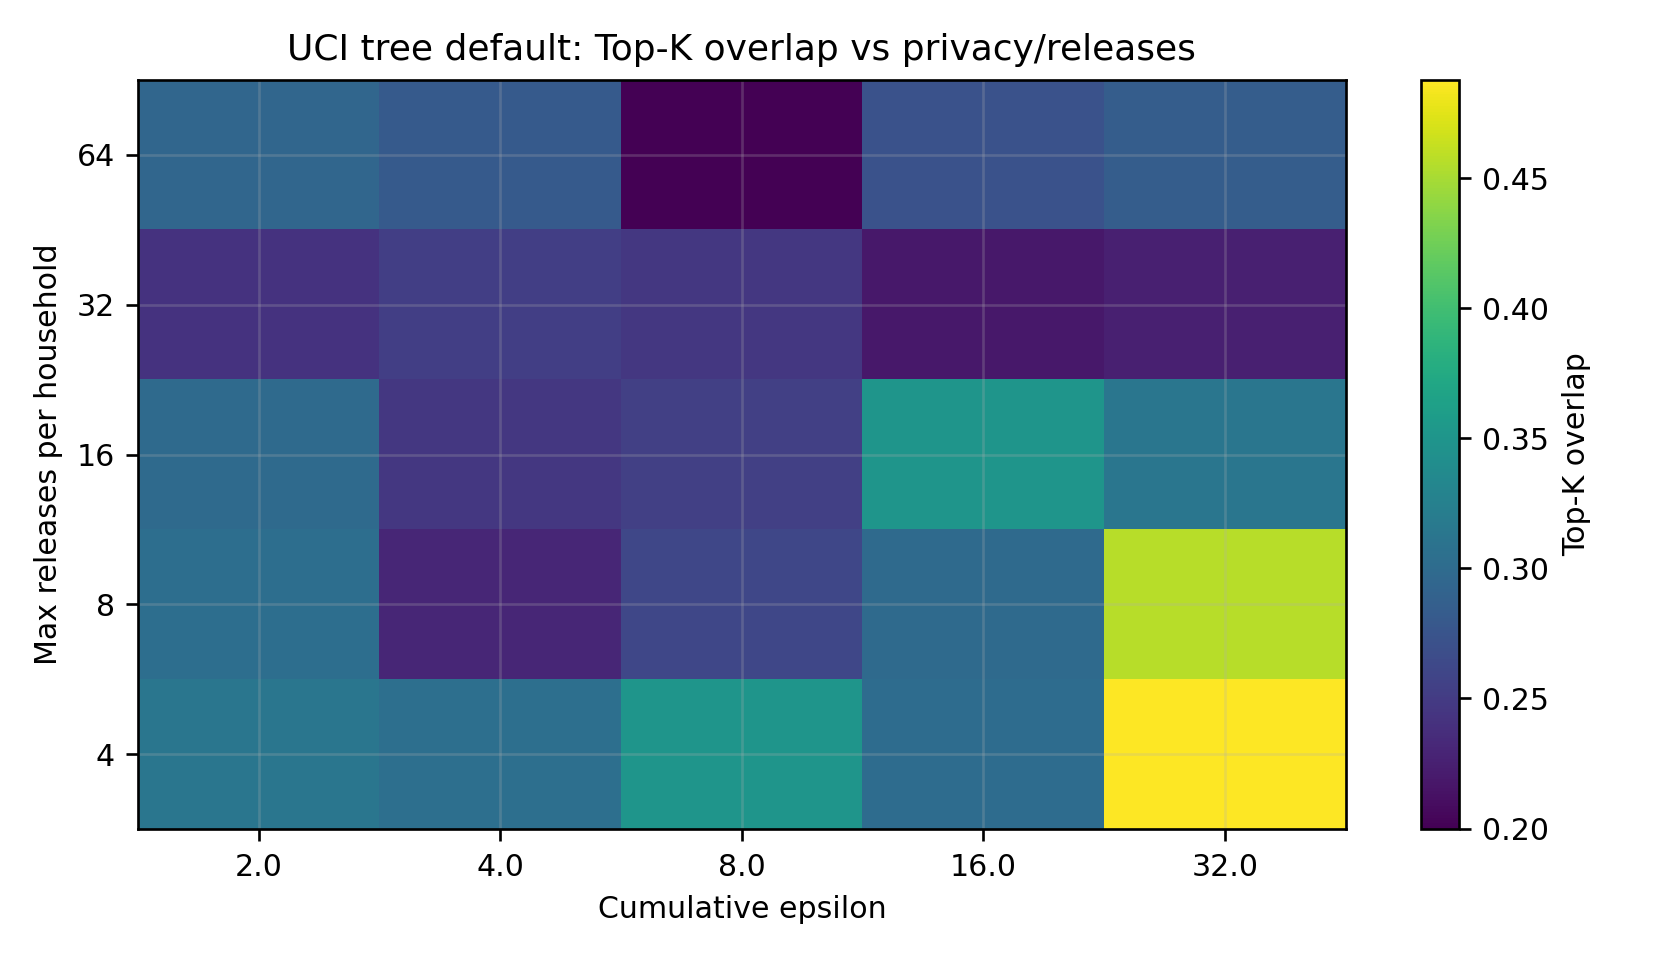
\includegraphics[width=\linewidth]{uci_tree_default_privacy_sweep_topk_overlap.png}\\[-1mm]
{\scriptsize (b) UCI}
\end{minipage}
\caption{Privacy-release sweep: Top-$K$ versus the allowed private-release cap
for $\epsilon\in\{2,4,8,16,32\}$. More releases increase service opportunities,
but the same horizon privacy budget must be spread across more releases, so
fidelity is non-monotone. Full cosine, recall, traffic, and privacy curves are
reported in the accompanying reproducibility appendix.}
\label{fig:frontier}
\end{figure*}

At $\epsilon=32$, OPSD moves from 8.4\% critical coverage and Top-$K$
0.377 at $M=4$ to 83.0\% coverage and Top-$K$ 0.287 at $M=64$; $M=16$
provides 31.1\% coverage with Top-$K$ 0.375. UCI moves from 10.3\%
coverage/0.488 Top-$K$ at $M=4$ to 53.5\%/0.284 at $M=64$. Thus coverage
can be increased, but not for free under a fixed horizon privacy budget.

\subsection{Interpretation and limitations}

The results support a communications contribution: a privacy-aware
semantic packet layer plus adaptive scheduling can sharply reduce
operator-facing XAI traffic while respecting cumulative household
privacy and endpoint fairness. They do \emph{not} support the claim that
high-recall automated intervention is solved. The M8 policy is
conservative; its mean critical-event recall is 3.7\%. Low false
intervention and high precision must therefore be interpreted together
with the 7.8\% mean critical-event coverage. The release sweep shows how
coverage can be increased, but also why doing so under a fixed
full-horizon privacy budget can destroy attribution signal.

Further limitations are the synthetic zone hierarchy and the
scheduler-level wireless abstraction. The privacy theorem protects
packet contents under the stated household adjacency, not arbitrary
traffic-analysis side channels. Physical feeder topology, link-level or
field traces, and event-window/daily privacy accounting are important
next validation steps. The present contribution is the joint design and
its measured feasibility boundary, not a claim of deployment-complete
grid control.

\paragraph{Extended analysis.}
A reader-facing supplementary report contains the complete 72-condition
v19 M8 means, all paired comparisons, M4--M8 sensitivity, temporal-regime
analysis, the full feasibility ladder, the 50-setting privacy--release
sweep, validation metadata, and result-by-result discussion. It is not
required for any claim made here and can be provided by the authors upon
request.

\section{Conclusion}

We presented \method{} as a two-layer private explanation-delivery
framework rather than a competition between two proposed methods.
\mapxai{} provides the privacy-accounted semantic representation;
\method{} schedules those modes under wireless, deadline, freshness,
criticality, fairness, and remaining-privacy constraints. In 720 paired
runs, the proposed stack has no privacy-budget violations and reduces
traffic by 79.4--94.6\% relative to external full/fixed-DP policies at a
conservative selective-release operating point. The feasibility ladder
identifies cumulative household-level DP as the dominant explanation
bottleneck, while compression contributes little additional loss. This
finding changes the design priority: future gains should come from
careful private-release timing and privacy-horizon design, not simply
from more aggressive explanation compression or scheduler retuning.

\begin{thebibliography}{00}

\bibitem{dwork2006calibrating}
C. Dwork, F. McSherry, K. Nissim, and A. Smith, ``Calibrating noise to
sensitivity in private data analysis,'' in \emph{Theory of Cryptography},
LNCS, vol. 3876, Springer, 2006, pp. 265--284.

\bibitem{mironov2017rdp}
I. Mironov, ``R\'enyi differential privacy,'' in \emph{Proc. IEEE CSF},
2017, pp. 263--275.

\bibitem{lundberg2017shap}
S. M. Lundberg and S.-I. Lee, ``A unified approach to interpreting model
predictions,'' in \emph{Advances in Neural Information Processing
Systems}, vol. 30, 2017, pp. 4765--4774.

\bibitem{sundararajan2017ig}
M. Sundararajan, A. Taly, and Q. Yan, ``Axiomatic attribution for deep
networks,'' in \emph{Proc. ICML}, PMLR, vol. 70, 2017, pp. 3319--3328.

\bibitem{kaul2012aoi}
S. Kaul, R. Yates, and M. Gruteser, ``Real-time status: How often should
one update?'' in \emph{Proc. IEEE INFOCOM}, 2012, pp. 2731--2735.

\bibitem{gholizade2026fedxai}
M. Gholizade, F. Ruffini, P. Ducange, and F. Marcelloni, ``Federated
explainable artificial intelligence: Roles, architectures, evaluation,
and open challenges,'' \emph{Expert Systems with Applications}, vol. 331,
Art. no. 133183, 2026.

\bibitem{li2026fedsva}
Y. Li, J. Gui, and Y. Wu, ``Towards explainable privacy preservation in
federated learning via Shapley value-guided noise injection,'' in
\emph{Proc. IEEE ICASSP}, 2026, doi: 10.1109/ICASSP55912.2026.11464062.

\bibitem{piran2025privatedfl}
F. J. Piran, Z. Chen, Y. Zhang, Q. Zhou, J. Tang, and F. Imani,
``Privacy-preserving decentralized federated learning via explainable
adaptive differential privacy,'' arXiv:2509.10691, 2025.

\bibitem{opsd2020household}
Open Power System Data, ``Household data,'' version 2020-04-15, 2020.
[Online]. Available:
\url{https://data.open-power-system-data.org/household_data/2020-04-15/}

\bibitem{uci2015eld}
A. Trindade, ``ElectricityLoadDiagrams20112014,'' UCI Machine Learning
Repository, 2015, doi: 10.24432/C58C86.

\bibitem{3gpp38901}
3GPP, ``Study on channel model for frequencies from 0.5 to 100 GHz,''
3GPP TR 38.901, version 18.1.0, Release 18, Feb. 2026.

\bibitem{bolstad2022load}
D. A. Bolstad, U. Cali, M. Kuzlu, and U. Halden, ``Day-ahead load
forecasting using explainable artificial intelligence,'' in
\emph{Proc. IEEE ISGT}, 2022, pp. 1--5.

\bibitem{wu2022load}
K. Wu, J. Gu, L. Meng, H. Wen, and J. Ma, ``An explainable framework
for load forecasting of a regional integrated energy system,''
\emph{Protection and Control of Modern Power Systems}, vol. 7, no. 1,
Art. no. 24, 2022.

\bibitem{kruse2021frequency}
J. Kruse, B. Sch\"afer, and D. Witthaut, ``Revealing drivers and risks
for power grid frequency stability with explainable AI,'' \emph{Patterns},
vol. 2, no. 11, Art. no. 100365, 2021.

\bibitem{gebhard2025anomaly}
T. Gebhard, A. Tundis, and F. Steinke, ``Explainable anomaly detection
for grid monitoring using probabilistic load forecasting,'' in
\emph{Proc. IEEE SmartGridComm}, 2025.

\bibitem{baur2024loadxai}
L. Baur, K. Ditschuneit, M. Schambach, C. Kaymakci, T. Wollmann, and
A. Sauer, ``Explainability and interpretability in electric load
forecasting using machine learning techniques---A review,'' \emph{Energy
and AI}, vol. 16, Art. no. 100358, 2024.

\bibitem{shokri2021privacy}
R. Shokri, M. Strobel, and Y. Zick, ``On the privacy risks of model
explanations,'' in \emph{Proc. AAAI/ACM AIES}, 2021, pp. 231--241.

\bibitem{yates2019aoi}
R. D. Yates, Y. Sun, D. R. Brown, S. K. Kaul, E. Modiano, and S. Ulukus,
``Age of information: An introduction and survey,'' \emph{IEEE J. Sel.
Areas Commun.}, vol. 39, no. 5, pp. 1183--1210, 2021.

\bibitem{ma2023semantic}
Z. Qin, X. Tao, J. Lu, W. Tong, and G. Y. Li, ``Semantic communications:
Principles and challenges,'' arXiv:2201.01389, 2022.

\bibitem{jain1984fairness}
R. Jain, D.-M. Chiu, and W. Hawe, ``A quantitative measure of fairness
and discrimination for resource allocation in shared computer systems,''
DEC Research Report TR-301, 1984.

\end{thebibliography}

\end{document}
